%!TEX root = ../thesis.tex

%\chapter{Synthesis and outlook} 
\chapter{Concluding remarks} 
\label{chapter:conclusion} 

\ifpdf
    \graphicspath{{Conclusion/Figs/Raster/}{Conclusion/Figs/PDF/}{Conclusion/Figs/}}
\else
    \graphicspath{{Conclusion/Figs/Vector/}{Conclusion/Figs/}}
\fi


\begin{pquotation}{\textsc{David Berman, \textit{The Natural Bridge}, 1996}}
What if life is just some hard equation? \\
On a chalkboard in a science class for ghosts \ldots
\end{pquotation}


\section{Summary}

The key scientific contributions made by this thesis can be summarised as follows:

\begin{itemize}

\item On rocky planets several times Earth's mass, topography models show a rather narrow window, in terms of surface water mass fraction, that permits land masses emerging from oceans. %Surprisingly, the absolute volume of water that could be contained below topographic highs decreases as planet size increases, even though larger planets have more surface area. 
Therefore Earth's land/ocean fraction $\in (0,1)$ does not seem like a common outcome across planets in general.

\item An Earth-sized stagnant lid planet, despite having high mantle melting rates, is shown to have lower mantle outgassing rates compared to modern Earth. If the mantle is also comparatively more reducing, then the outgassing rates of \ce{CO2}, CO, and \ce{H2O} start to drop off even further. %I go on to suggest that, with some assumptions about their rates of removal from the atmosphere, it is not inevitable that the key volcanic greenhouse gases \ce{CO2} and \ce{H2O} were abundant enough in the Archean atmosphere to make up for the fainter young sun; conversely, geochemical evidence for temperate conditions in the Archean would suggest that our stagnant lid model does not describe the style of convection and outgassing on Archean Earth.

\item The maximum concentrations of water that planets can sequester in their rocky mantles are predicted as a function of planet mass, across %the range of 
realistic mineralogies expected for exoplanets. Constrained here for the first time, these values are key initial conditions for thermal history models. %, given that water has a critical role in several mantle convection processes. 
The most massive rocky planets may have limited deep water cycles due to relatively thin upper mantles, insofar as the top of the lower mantle is universally dry. 

\item Upper mantle oxygen fugacities will necessarily differ across exoplanets by at least $\sim$3~dex. This minimum variability is due only to variability in mineral phase equilibria and is constrained by host star refractory abundances.  %Assumed differences in ferric iron budgets can then add at least several more dex of oxygen fugacity variation. 
%Because some atmospheric gases can have both volcanic and biogenic origins, 
I give a reason for why we might do well to appreciate the intrinsic variability of exoplanet mantle oxygen fugacities, which ultimately control gas mixing ratios in volcanic atmospheres.

\end{itemize}



%\section{Synthesis: Water and habitability}
\subsection{On water and habitability}

\begin{figure}
  \centering
  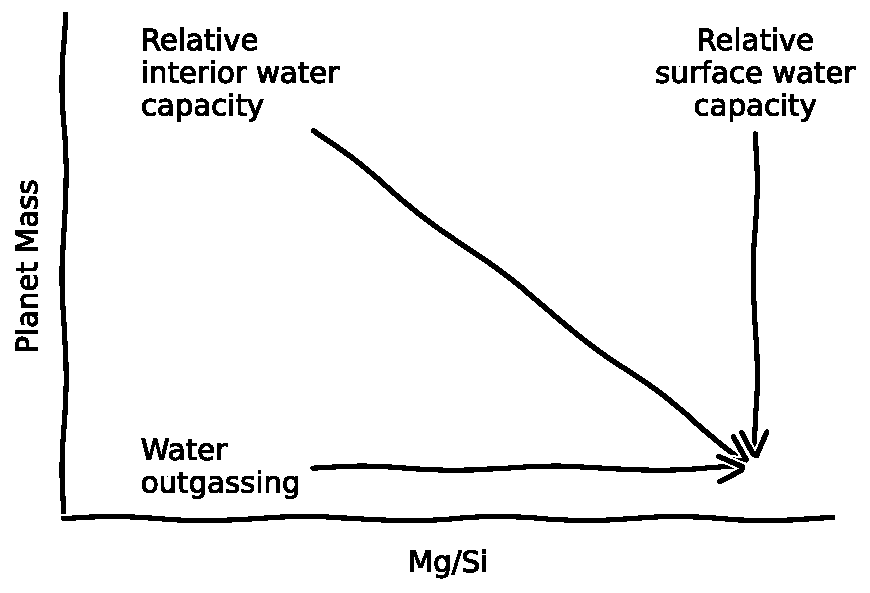
\includegraphics[width=0.66\linewidth]{summary}
\caption[Summary cartoon of water on rocky planets in the context of their mass and compositional diversity.]{Water on rocky planets contextualised within this thesis' overarching themes of planetary mass and compositional diversity. Arrows show proposed trends of increasing water content.}
\label{fig:surfacewater}
\end{figure}


%\todo{show plot with water and topography --- but what are the limits to predicting surface water? not just modelling outgassing because the atmosphere is really important. cf. Ana Lobo paper, yoshi miyazaki stuff... won't just condense into an ocean reliably}


The classic definition of planetary habitabilty is based on the stability of liquid water \citep{kasting_habitable_1993}. Much of the work presented in this thesis is, indirectly or directly and not-entirely-by-accident, related to where a planet's water is. It might therefore be interesting to place the preceding chapters in a retrospective watery framework. Here we can adopt the paradigm that virtually all of a rocky planet's total water mass will be partitioned between two reservoirs, its surface oceans and its mantle. In Chapters \ref{chapter:topography} and \ref{chapter:rockywater}, I predicted the capacity of these reservoirs respectively. In Chapter \ref{chapter:outgassing}, I predicted the flux of water between them, under certain conditions. Finally, in Chapter \ref{chapter:fo2}, I put constraints on the distribution of the most influential single parameter (cf. Fig. \ref{fig:corr}) affecting this flux; that is, \fo. Taking the results of these works together within the two main axes of rocky planet diversity introduced in Chapter \ref{chapter:intro}, some general trends in planetary water contents might be proposed (Fig. \ref{fig:surfacewater}).


With that said, I should stress that these four studies were not designed to be cognitively coupled in this way; i.e., to make rigorous predictions about how water flows through and on top of planets in general. Importantly, the actual presence of surface water on a planet is not guaranteed, even if the planet is in the circumstellar habitable zone of water stability, and even if it is endowed with water from formation. Whether or not a rocky planet can ultimately build and maintain surface oceans will be determined by its instantaneous atmospheric conditions as much as its interior conditions. For example, a certain minimum atmospheric partial pressure of water vapour is needed if water condensation is to proceed at all, which depends on the surface temperature and \ce{CO2} partial pressure \citep{miyazaki_inefficient_2022, miyazaki_wet_2022}. Models of atmosphere dynamics have revealed complex patterns of surface water loss on rocky planets \citep[e.g.,][]{lobo_terminator_2023}; these processes may ultimately need to be considered if we hope to make some predictions about planetary habitability, in this classical sense of the word. 


\section{Outlook}

\subsection{Parameter uncertainty}

All (exo)planetary interior modelling has been limited by the available data. There are three obvious areas where more or higher-quality data would directly advance our field.


\subsubsection{High-precision abundance measurements of planet-hosting stars and white dwarfs}


The uncertainty on stellar abundances is still too high to delimit individual exoplanets according to mineralogical ``populations''. This abundance data must be an order of magnitude more precise (1/1000 dex) if we are to make meaningful inferences about a given planet's mantle mineral modes \citep{hinkel_star_2018}. High-precision measurements of stellar Fe abundances are necessary to place upper limits on an exoplanet's metal core size, and therefore constrain its interior structure, maximum volatile-envelope mass fraction, and nominal likelihood of being rocky (\citealt{schulze_probability_2020, unterborn_nominal_2023}, cf. Fig. \ref{fig:compositional-link}). Lastly, a larger sample of high-precision abundances in polluted white dwarfs will be vital to test empirically how the refractory element ratios of planets are modulated from those of their host stars (cf. Fig. \ref{fig:hypatia_vs_pwd}): the omnipresent working hypothesis in all studies of rocky planet interior compositions. 


As I discussed in Chapter \ref{chapter:intro}, much of the error on FGKM star abundances is due to different data reduction techniques between researchers, as opposed to actual measurement error introduced by our instrumentation. The observational astrophysics community is making efforts to understand why this disagreement exists, and to find steps to minimise it \citep{hinkel_comparison_2016}. Notably, individual groups have been reporting abundances at this precision for nearly a decade \citep[e.g.,][]{ramirez_chemical_2014, nissen_highprecision_2015, spina_planet_2016}; it does not seem impossible to achieve more widely in the near future. Any interpretation of the white dwarf data hinges on our theoretical understanding of these bodies' accretion dynamics, but this is an area of active research \citep[e.g.,][]{harrison_bayesian_2021, buchan_planets_2022, brouwers_asynchronous_2022, brouwers_asynchronous_2023}.


\subsubsection{High-pressure mineral data}

We do not understand the behaviour of minerals at high mantle pressures perhaps as well as we would like to. Predictions of the interior structures of massive rocky planets are limited by uncertainties in the equations of state parameters and phase equilibria of silicates, especially above $\gtrsim$0.5 TPa. However, even if the highest pressures are a challenge to reach in laboratory settings, first-principles methods (e.g., density functional theory) have already proven vital in data generation \citep[e.g.,][]{umemoto_twostage_2011, tackley_mantle_2013, sakai_experimental_2016, umemoto_phase_2017}. %das_highpressure_2020, kovacevic_miscibility_2022, li_ultrahighpressure_2022}.


Beyond equations of state, it is also necessary that we constrain other material properties relevant for mantle thermal evolution: namely, viscosities and melting temperatures. These data are incomplete across exoplanet parameter space even at lower pressures, since most experimental petrology work so far has not necessarily needed to perform measurements across extraterrestrial mantle compositions. Even a null result (i.e., a negligible dependence) would be immensely useful. A systematic effect of Mg/Si on viscosity, assuming one can be found, could easily be adopted into convection models \citep{spaargaren_influence_2020}---this example is salient because planetary Mg/Si distributions might be measureable.

For example, where Chapter \ref{chapter:rockywater} adopted certain fiducial values of the water capacities of perovskite, stishovite, davemaoite, postperovskite \textit{etc.}, with better data in the future I anticipate that these results will be revised. In particular, the pressure-dependence of these phases' water capacities needs to be determined. \citet{deng_water_2022}, in a conference proceeding, present preliminary calculations of the water capacity of bridgmanite using molecular dynamics simulations and machine learning, the formal publication of which I am currently awaiting.




% although this has so far not succeeded, this could provide agreed-upon parameters that go into viscosity laws for a mantle in terms of temperature, pressure, mg/si, and water content




\subsubsection{The surface composition of Venus}

The solar system has another Earth-mass planet. Yet apart from the obviously hellish climate, we know hardly anything about its geology. Previous observations of our sister planet's surface emissivity have appeared consistent with felsic crustal rocks, which, intriguingly, would crystallise in the presence of water similar to Earth's granite continents \citep{hashimoto_felsic_2008}. Planned space missions VERITAS and EnVision (set with 2030s launch dates if not indefinitely delayed) would finally map the surface mineralogy of Venus. Given that Venus' bulk mantle mineralogy is expected to be very similar to Earth's, understanding how different the derived crusts are between the two planets would be an invaluable data point, if we are to ever understand the range of crustal compositions of exoplanets. These missions would also provide needed insight into Venus' enigmatic tectonic style, aiding our confidence in modelling the thermal histories of Venus-like exoplanets. 

As a note, the existence of Venus proves that planets are not pushed down pre-determined evolutionary tracks according to their position in Mg/Si--$M_p$ parameter space. The major question, ``why are Venus and Earth different today?'', would not have a simple answer, but any progress towards it is progress towards understanding planets.


\nomenclature[z-v]{VERITAS}{Venus Emissivity, Radio science, InSAR, Topography, And Spectroscopy}

\subsection{Model uncertainty}


Apart from minimising uncertainty on the input data, the other direction for future work attends to the infrastructure of models itself. Fast, simple 1D thermal history models are probably our best tool for exploring exoplanet parameter space. However, these models must capture the necessary physics. Sometimes higher-resolution 2D or 3D models can find certain insights into nonlinear processes that 1D models cannot. Melting rate estimates are a special challenge in 1D due to this nonlinearity (e.g., local melting depends on the history of previous melting, Chapter \ref{chapter:outgassing}; see also a review by \citealt{katz_physics_2022}). As such, a useful calculation would be to quantify the discrepancy in absolute melt volumes between high-resolution numerical models \citep[e.g.,][]{noack_volcanism_2017} and contemporary 1D models \citep[e.g.,][]{spaargaren_influence_2020, baumeister_redox_2023}, all else equal. I note that there are some good parameterisations of mantle melting in existence \citep[e.g.,][]{katz_new_2003}, but seemingly no unified method for applying them at planetary scales. Previous 1D studies of exoplanet mantle outgassing \citep[e.g.,][]{liggins_growth_2022} have plugged in constant values of numerically-calculated planetary melting rates from the literature, but by nature this approach cannot capture time-dependence or nonlinearity \citep[cf.][]{keller_statistical_2012}, and are of course stuck in nominal tectonic regimes, compositionally-dependent rheologies and solidii, \textit{etc}. 

Nevertheless, fully-coupled 1D thermal history models, which track water dynamics and their effects on mantle melting and viscosity, have demonstrated recent success resolving some old issues about Earth's thermal history \citep{seales_buffering_2022}. Thus, if we have melting implementations we can believe in, especially now that initial conditions for mantle water content are offered (Chapter \ref{chapter:rockywater}), we might apply 1D models of mantle convection to put realistic constraints on the expected range of---as per a theme of this thesis---\ce{H2O} outgassing fluxes on rocky planets, as a function of their (observeable) mass, age, and host star composition. Fluxes of \ce{CO2} are a natural extension \citep[see][]{lehmer_carbonatesilicate_2020}, being a key hurdle in predicting the climate states of planets in the circumstellar habitable zone \citep[e.g.,][]{graham_co2_2022}, although the geochemistry governing carbon's storage and transport in the mantle is distinct from that of water \citep{dasgupta_ingassing_2013}. From there we can address the expected variety of planetary climates within the circumstellar habitable zone, naturally feeding estimations of the frequency of truly Earth-like planets, laying the groundwork for a statistical understanding of Earth’s cosmic station.




%\todo{coupled 1D models involving water transport, its effects on melting and viscosity, have demonstrated recent success in possibly resolving some old issues about earth's thermal history \citep{seales_buffering_2022}, and these considerations are simple enough and clearly justified to go into future 1D thermal models for exoplanets, now that I have provided initial conditions }


%\todo{in need of new scaling laws for melting rates, or a distribution of melting rates, that can slot into parameterised models, in particular of stagnant lid planets. these could be obtained from numerical experiments }




%TTFN!